%% The CSAIL abstract book is a custom document class called 
%% "csailabstractbook".  It is based on the teTeX 1.0 distribution of LaTeX,
%% insofar as it uses a number of additional packages from teTeX for its
%% behind-the-scenes formatting. If you are using a different
%% distribution of LaTeX, it is possible that your distribution does not
%% have the necessary packages, in which case you will receive a missing 
%% package error when using the class file. You may wish to latex a copy 
%% of this file as-is to ensure that your configuration is correct.  

%% You should *not* include additional packages in preparing your
%% abstract.  The csailabstractbook class automatically includes the
%% standard "graphicx" package for inclusion of figures. An example of
%% its syntax is given in the text below, and more detailed documentation
%% can be found from the lab's latex page. Please use PDF files for your images.

%% Producing your abstract should be straightforward. Keeping all your
%% files in your working directory, run latex on the abstract file, bibtex
%% on the abstract file, and then latex on the abstract file twice.

\documentclass{csailabstractbook}

\begin{document}

%% The use of the sectioning commands, \abstitle and \absection, should 
%% be clear.  Try to follow the form of the sample text below, except
%% that your text should make a bit more sense.  It is ok to delete a 
%% section if it doesn't apply to your work.


\abstitle{Hybrid Space-Time Partitioning of Stream Programs with
Linear Code Generation for Raw}
         {Michael Gordon, Jasper Lin, William Thies, and Saman Amarasinghe}

%% Please include an index entry for each author, keeping the names
%% consistent across abstracts. 
\index{Gordon, Michael}
\index{Thies, William}
\index{Lin, Jasper}
\index{Amarasinghe, Saman}

\absection{What}
We are developing compiler technology for the StreamIt programming
language~\cite{streamitcc}, a high-level stream language that aims to
be portable across communication-exposed machines.  StreamIt contains
basic constructs that expose the parallelism and communication of
streaming applications without depending on the topology or
granularity of the underlying architecture.  Our previous work
\cite{streamit-asplos} has focused on 
implementing a {\it space-multiplexing} (see below) backend for
MIT's Raw architecture \cite{raw}, a tiled architecture 
with fine-grained, programmable communication between processors.
Currently we are implementing a new backend targeting Raw that will
incorporate the lessons learned while investigating our previous work.

\absection{Why}
As we approach the billion-transistor era, a number of emerging
architectures are addressing the wire delay problem by replicating the
basic processing unit and exposing the communication between units to
a software layer.  These machines are especially well-suited for
streaming applications that have regular communication patterns and
widespread parallelism.  However, today's communication-exposed
architectures are lacking a portable programming model.  If these
machines are to be widely used, it is imperative that one be able to
write a program once, in a high-level language, and rely on a compiler
to produce an efficient executable on any of the candidate targets.

\absection{How} 

Given a stream graph, composed of filters (actors) and FIFO,
uni-directional arcs connecting the filters, what is the best way to
execute it?  If we are targeting a uniprocessor, the most obvious
technique would be {\it time multiplexing} where we run one filter at
a time on the processor.  Load balancing is not an issue and the
memory interface provides synchronization.  Problems arise if we
target a multiprocessor.  Time multiplexing leads to long latency,
lots of memory traffic (possibly with bad cache behavior), and the
utilization would depend on the presence of data-parallel filters that
could be spread across the chip.

A second approach would be to run all the filters in parallel, each on
its own tile.  This is termed {\it space multiplexing}.  Our first 
StreamIt compiler for Raw uses this technique.  Space multiplexing
affords no filter swapping overhead, reduced memory traffic,
localized communication, and tighter latencies.  Due to these
properties, space multiplexing scales extremely well.  
Load balancing is the performance focal point of space multiplexing.  Merging
and splitting filters of the stream graph until the graph is composed
of $n$ load balanced filters, where $n <=$ \# of processing
elements, proved difficult, with many factors coming into play.  
Further, constraining ourselves to space multiplexing forced us to
need to support arbitrarily complex communication patterns.

The technique employed by our new backend for Raw is to merge the
advantages of space multiplexing and time multiplexing.  This hybrid
approach will time multiplex different groups of filters and space
multiplex the filters within a group. We call each group a space-time
slice or just a slice.  Hybrid space-time multiplexing allows space
multiplexing for fine-grained, systolic sections of the stream graph
 and time
multiplexing for improved load balancing.  Furthermore, we use
software pipelining techniques to allow arbitrary ordering of slices
during steady-state execution.

In \cite{lamb03} a linear analysis framework for StreamIt is
introduced.  We define a {\it linear} section of a stream graph as
groups of filters that compute a linear combination of their inputs.
Using this framework we can discover the linear sections of a
streaming application.  Many ubiquitous DSP kernels are linear
including FIR, low and high-pass filters, and DFT.  This linear
computation can be represented as a matrix multiplication and
efficiently mapped to Raw.  Currently, linear slices of the stream
graph are space multiplexed across tiles of the chip using
parameterized computation and communication code.  The matrix
representations of the linear filters are broken into pieces
that the compiler targets for aggressive code generation.  The
aggressive code generation results in optimal usage of the tiles
for each piece.

\begin{figure}[tbh]
	\vspace{-.2in}
  \centerline{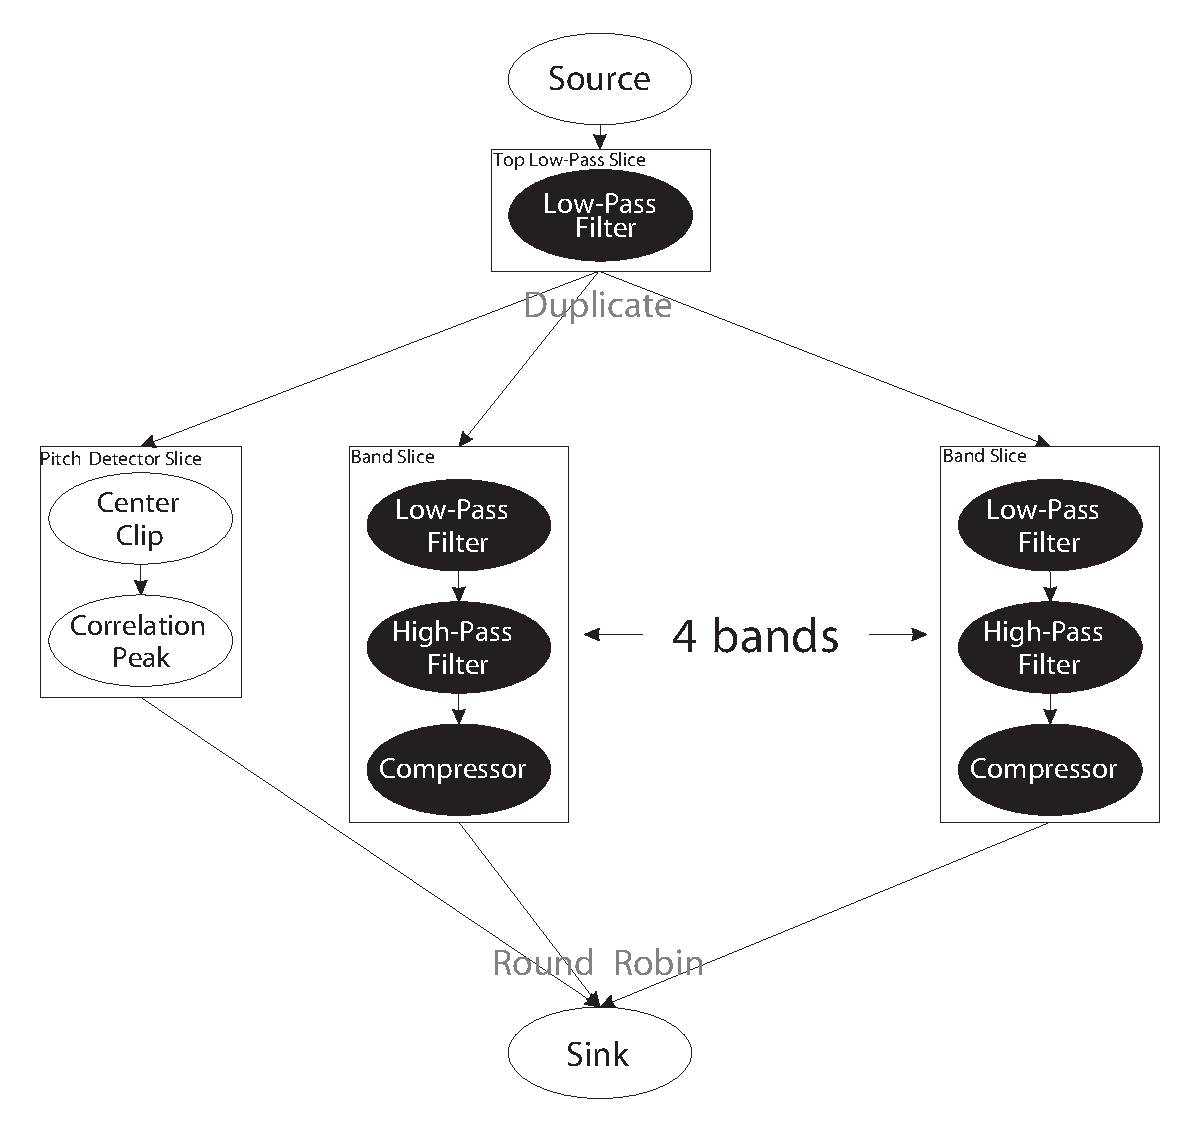
\includegraphics[width=3.0in]{mgordon_figure1.pdf}}
	\vspace{-.2in}
  \caption{The Stream Graph for the Channel Vocoder.}
	\vspace{-.2in}
  \label{streamgraph}
\end{figure}


   
We will now present a small example to solidify the reader's
understanding of our work.  In Figure \ref{streamgraph} we show the
stream graph for a simple channel vocoder.  The dark ovals denote
the linear filters of the application.  The white ovals are non-linear
but stateless filters and thus can be data-parallelized.  

An example mapping of this application would first execute the top
low-pass filter slice, occupying the entire Raw chip executing enough
times to supply the subsequent slices. Next, each band slice will
occupy a quarter of the chip, executing 4 bands in parallel.  Remember
that each of the above slices are linear and our parameterized linear
code generation provides near-optimal utilization. Finally, the
non-linear, stateless pitch detector slice is data-parallelized across
the entire Raw chip, reading its input from DRAM and writing its
output to DRAM.  Each slice reads its input from and writes its output
to off-chip DRAM.
 
\absection{Progress}
Currently, we have completed a first version of our hybrid space-time
multiplexing Raw backend for StreamIt and are in the process of
evaluating it's performance and scalability.  We have a robust
implementation of inter-slice communication using Raw's off-chip
streaming memory interface.  For intra-slice communication, we exploit
Raw's static network and we translate StreamIt's filter code into C
code to be executed on the compute processors.  We have completed
parameterized code generation for linear filters.   

As for the high-level algorithms, we have implemented a greedy
algorithm to partition and schedule the stream graph into ordered slices.
This algorithm has the freedom of producing an arbitrary ordering of slices
to best distribute the work evenly. It is the task of the software
pipelining algorithm to take in this schedule and produce a valid
execution by determining what executions are needed in the initialization
stage to prime the pipeline.

\absection{Future}
In the near future we would like to explore more advanced partitioning
and layout algorithms.  Additionally, we will further expand
space multiplexing by investigating additional parallelism schemes
such as filter fission (breaking a filter into multiple, smaller
filters), investigating optimizing additional filter representations
such as state-space, and implementing optimized linear code generation 
targeting sparse matrices.  We are working on a new intermediate representation
for our compiler that will allow us to directly generate assembly code for
Raw's compute processors. Generating our stream code in a procedural
framework is a source of many inefficiencies.  

\absection{Research Support}
This work is supported in part by a grant from DARPA (PCA
F29601-04-2-0166), awards from NSF (CISE EIA-0071841, ITR ACI-0325297,
NGS CNS-0305453), and a fellowship from the MIT-Oxygen Project.

%% The abstract bibliographies should be done using bibtex.  Please
%% compile your bibtex entries into a single file with a distinguishing
%% name. The \absbibliography command is analogous to the \bibliography
%% command, taking a single argument, the name of your bibtex file, 
%% minus the .bib extention. The \bibliographystyle command should not
%% be used.  You can use a single bibliography file if you are submitting
%% multiple abstracts.  

\absbibliography{mgordon_bib}

\end{document}
